\documentclass[a4paper]{article}

\addtolength{\textwidth}{40mm}
\addtolength{\oddsidemargin}{-20mm}
\addtolength{\textheight}{40mm}
\addtolength{\topmargin}{-20mm}

\usepackage{ifpdf}
\usepackage{subfigure}
\usepackage{epsfig}

\title{\LARGE \bf
Alternative waterfall
}
\author{Chris Nicholls, Irina Voiculescu and Stuart Golodetz
}
\date{Oxford University Computing Laboratory}

\begin{document}

\maketitle
\thispagestyle{empty}
\pagestyle{plain}



There are many applications for image segmentation in the world of
medical imaging, for example, feature identification and
classification, 3D visualisation, and volume estimation. All these
help when working with CAT scans and each require knowledge of where
key anatomical features are found in the image.

In order to locate any such features, the image needs to be
segmented. That is, pixels of similar greyscale values get grouped
together in one region. Most algorithms tend to over-segment images
significantly, leading to far more regions than can be handled
sensibly. This effect is partly due to problems such as indistinct
boundaries between features and the variation present between
different images, and partly due to the algorithms not having any
knowledge of the context in which the segmentation takes place.

%---
\begin{figure}
\centering
\ifpdf
        {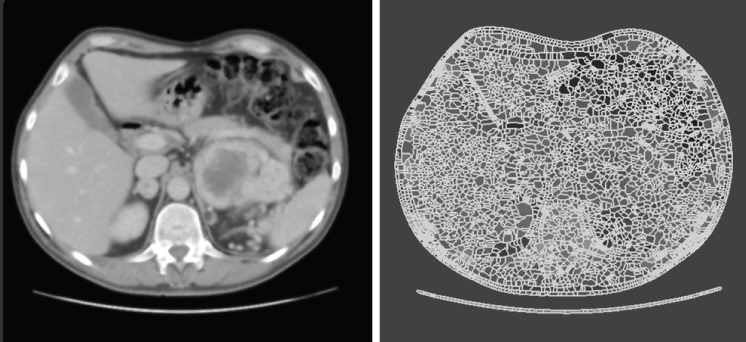
\epsfig{file=oversegmentedimage.png, height=.2\linewidth}}%
\else
        % TODO
\fi
\caption{Example of oversegmented image}
\label{fig:oversegmented}
\end{figure}
%---

Figure~\ref{fig:oversegmented} illustrates (on a CAT scan) the results
of a common segmentation algorithm, the watershed. The image is
clearly over-segmented and hence not much more useful than the
original for the purposes mentioned earlier.

This over-segmented image can be processed further by grouping
together those regions that feature similar grey values. This
technique is known as the waterfall algorithm. It yields a hierarchy
called a partition forest, which is a more comprehensive data
structure that can be used subsequently in the process of feature
identification. The waterfall algorithm is widely used and can produce
good results.

%---
\begin{figure}
\centering
\ifpdf
        {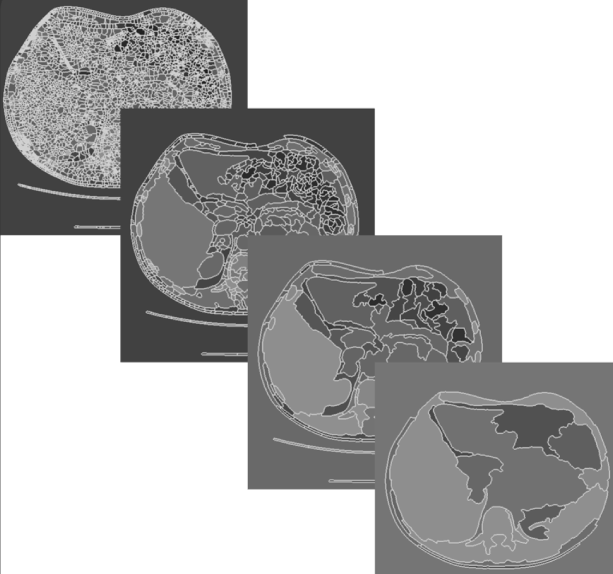
\epsfig{file=partitionhierarchy_4.png, height=.5\linewidth}}%
\else
        % TODO
\fi
\caption{Hierarchy of segmentations}
\label{fig:waterfall}
\end{figure}
%---

Figure~\ref{fig:waterfall} illustrates the various layers that result
from applying the waterfall algorithm repeatedly to the segmentation
shown in Figure~\ref{fig:oversegmented}.

Both the watershed and the waterfall algorithms are based on a
geographical metaphor. The image is regarded as a landscape, with each
grey value being associated to a terrain height. The valleys are in
the darker areas, whereas the lighter areas are regarded as peaks.

The waterfall algorithm~\cite{beucher, marcotegui} can be imagined as a flooding
process. The water falls into (low) catchment basins and gradually
fills them up to the nearest boundaries. When two adjacent basins have
been filled up to the boundary between them, they get joined (and the
boundary gets removed). This process continues until the whole image
becomes a single basin. The intermediate stages of the process can be
regarded as intermediate segmentations of the image, with each basin
representing a region, and each inter-basin peak representing a
boundary between regions.

The traditional implementation of this algorithm \cite{marcotegui} involves the
construction of a Minimum Spanning Tree (MST) and the gradual elision
of some of its edges. Its nodes are the local minima and maxima of the
plateaus in the landscape, whereas its edges are the relative
difference in height between these. (In actual fact it is the
landscape formed by the gradient of the original image that is used,
rather than the raw image.)

The collection of regional minimum edges of a graph $G$ is a connected
subgraph of $G$ whose edges have the same weight as each other, and
whose adjacent edges in $G$ have strictly higher weights. The
waterfall algorithm relies heavily on finding these regional minimum
edges, eliding them and rebuilding the MST -- a process which not only
requires careful implementation of the MST but, more importantly, is
relatively complex and hard to implement.

In this paper we present a new data structure for the waterfall
algorithm that simplifies the process and improves efficiency compared
to current implementations. It is based on a recursive-tree data
structure and a recursive relation on the nodes rather than the
conventional iterative transformations.

[some details about the new data structure]

Production of partition forests has many applications outside of the
field of medical imaging, for instance, binary space partitioning in
3D map rendering for games.

[some results, and possibly something about validation]

\begin{thebibliography}{2}

\bibitem{beucher}{Serge Beucher. {\em Watershed, hierarchical
    segmentation and waterfall algorithm}. In Mathematical Morphology
  and its Applications to Image Processing, Proc.\ ISMM 94, pages
  69-76, Fontainebleau, France, 1994. Kluwer Ac. Publ.}

\bibitem{marcotegui}{Beatriz Marcotegui and Serge Beucher, {\em Fast
    Implementation of Waterfall Based on Graph}. In Mathematical
  Morphology: 40 Years On, Springer Netherlands, 2005.}

\end{thebibliography}

\end{document}
